\subsection{Power System}
This section will look at the overall design that will power the nodes in the Aether Sensing Network. The Aether nodes will consist of a solar panel capable of powering the system while also charging the Lithium-Ion battery that will be used if the load demand exceeds the capabilities of the solar panel. Additionally, the node will be equipped with a USB port to charge the battery and power the system as a second option. This gives users of the design the flexibility to directly charge a depleted battery and maintain the system operational in situations where the solar panel cannot provide sufficient power. A battery charge management controller will be responsible for a voltage proportional charge control feature that will optimize the solar cell and will also allow the USB input to power the system. At the output end of the charge controller will be a linear dropout regulator (LDO) to drop down the voltage to a constant 3.3V which will be used as the main power line for the system.

\subsubsection{Overall Features}
A 3.7 V/4.2 V Lithium-Ion battery will be the main battery source in this design. The battery can be charged through one of 3 methods:
\begin{itemize}
    \item A 6V solar panel
    \item USB Input
    \item A 5V DC adapter in place of the solar panel
\end{itemize}

The design incorporates automatic charging current tracking through the battery charge management controller IC. This allows the system to operate at high efficiencies with solar panels of varying wattages. Three LED's will be used to indicate battery charge status to the user. The orange LED indicates the battery capacity is low and it’s charging; the green LED indicates the battery has been fully charged; the red LED indicates power is good and the system is on. A maximum charge rate of 500 mA is outputted by the charge controller and it is adjustable from 50 mA to up to a 1A charge rate. Our system is designed to draw the most amount of current possible, depending on the set maximum charge rate, from the solar panel to meet load requirements. If the load requires more current it will then turn to the battery. This smart load sharing automatically uses input power if available which prevents the battery from frequently charging and discharging and therefore extending the battery life. Since the Aether nodes are also intended for outdoor use, battery temperature was a factor that needed to be considered. If the Lithium-ion battery temperature exceeds a certain limit, charging it could potentially be dangerous. Therefore, the design will include a 10 \kOhm NTC thermistor connected to the charge controller IC to monitor battery temperature and automatically stop charging the battery if temperature thresholds are met. 

\subsubsection{Solar Panel Charging}
The nodes in the Aether Sensing Network will use Voltaic Systems’ 5.5 W 6 V solar panel to charge and power the node. A DC jack input will be used to connect the solar panel to the system. Charging the system with a solar panel means a filtering capacitor will be needed to stabilize the solar panel. A relatively large 4700 microfarad capacitor will be used on the PCB for this design. The biggest question of this solar powered system was whether to incorporate Max Power Point Tracker (MPPT) into the design. MPPT works by monitoring the voltage and current output curves of the solar panel in order to maximize the total power output of the panel. Since the voltage and current outputs of a solar panel are dependent on the amount of light outside, solar panel readings need to be consistently monitored. Typically, MPPT is done through the use of DC/DC buck converters so when solar panel voltages vary the buck converter will maintain the current draw to maximize the power output of the solar panel. Although MPPT increase solar efficiency, there were some critical downsides if used in this power design. The first is that DC/DC converters would increase the cost of the design as well as the size and circuit complexity, while only providing a maximum of 30\% increase in efficiency to small voltage solar panels. Additionally, when compared to applications with small voltages and currents, MPPT is not much more efficient than a linear converter. A 6V panel responsible of charging an approximately 4V battery will have an MPPT around 5V, since the linear charger will have an input diode with a 0.5V dropout, the inefficiency of a DC/DC converter is about the same as that of the voltage dropout of the diode. Its for this reason that MPPT is often used in systems with 12V lead-acid batteries and very large solar panels requiring multiple chargers. If the panel voltage can be maintained at approximately 1 volt above the battery voltage and the current draw can be kept steady under 1 ampere, near-MPPT performance can be obtained with the right charge controller.

Unlike DC and USB power inputs, voltages and currents are constantly varying in solar panels. The instability of solar panels can cause issues with battery chargers as they constantly turn on and off while trying to draw excessive current from the solar panel causing the voltage to drop. A single solar cell has an open circuit voltage 0.5V when it is not drawing any current. As current begins to increase the voltage begins to collapse and reach 0V at the short circuit current for the solar cell. As light changes the battery charger begins to demand more current from the panel exceeding its short circuit current causing the voltage to collapse and the charger to turn off. Therefore, a charger capable of monitoring the voltage of the solar panel so that it does not demand current past the solar panels short circuit current is needed. With the right battery charger and the capacitor in place to further stabilize the solar panel solar optimization can be achieved. As shown in Figure \ref{fig:Solar-panel-connection}, the connection for the solar panel can be seen. A Schottky diode charges a 4700uF capacitor for the solar panel, the diode prevents any charge in the capacitor to drain back to the panel.

\begin{figure}
    \centering
    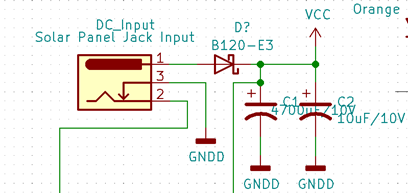
\includegraphics[width=5.5in]{figures/Solar Power Input.png}
    \caption{Schematic for Solar Panel DC Input}
    \label{fig:Solar-panel-connection} 
\end{figure}

\subsubsection{USB Power Input}
Aether nodes will also have the capability of being powered and charged through direct USB-C input. In certain conditions we have found having another potential source of power can come in handy. Namely in cases where solar power is no longer functional or in cases where we want to manually charge the battery. As a result, we have found USB charging the most efficient way to accomplish this. This design incorporates USB input to the MCP73871 main input pin. The system will operate depending on which power input is selected. The design will incorporate a USB-C input. This source of power is easy to construct, maintain, and also reliable. The node will take on power from a USB source where an IC will take in the power and effectively convert it to appropriate levels to supply the load and charge the battery alone or in conjunction with our solar source. While the chip is being supplied with the USB power, the MCP73871 will have additional precautions monitoring the output current to the battery and load ensuring there's over current protection from the USB power source. USB charging, on average, supplies its demand with 2.5 watts of power, should this be maintained through effective usage of the MCP73871 we could find months of charge on the battery in only a matter of hours while simultaneously powering our system.
\paragraph{}
The second major function of the USB-C power input is to serve as a communication link to the Lora-E5 micro controller. Not only has USB become a standard for charging devices but USB has also become an industry standard interface for transmitting data. The power design of this circuit will include a USB-C port connector connected to a USB-to-UART Bridge IC.  This IC is necessary since the Lora-E5 micro controller can only communicate through a UART protocol and not USB. A crucial factor to consider when adding a USB system that interfaces with an external environment such as in Aether, is electrostatic discharge (ESD) and other forms of electrical interference. The Aether power system design will feature an ESD protection circuit integrated with electromagnetic interference (EMI) protection as well. Protection circuitry will be vital to ensuring uninterrupted operation of the USB communication interface and providing ESD discharge robustness to the USB system. Although ESD risk are present throughout all USB systems, particular caution needed to be taken when using USB-C. The USB PD high power delivery in USB-C in addition to its smaller more compact design, place the system at more of ESD related issues. Protection circuitry also prevents damage to downstream components that may result from short circuitry between the connector’s adjacent VBUS and CC or SBU pins. There are several different circuit design methods that can be implemented for ESD and EMI protection. Aether's USB power design uses an integrated EMI suppression with ESD protection. The principle components used in this protection circuit are bidirectional TVS surge protection diodes, a choke filter, and capacitors. The TVS diodes are used to limit fast transients at low voltage levels while the choke filter attenuates high frequency and fast voltage peaks to protect against common-mode disturbances. When placed appropriately, capacitors play a crucial role in minimizing EMI in this design by forming low-pass filters bypassing the RF signal to ground. A 1A fuse is placed on the line out of VBUS to protect from over voltages. With the appropriate protection in place, the USB output of 5V can be sent to the charge controller circuit in to charge and power the system. The protection circuit designed can be seen in Figure \ref{fig:USB-Protection}. 

\begin{figure}
    \centering
    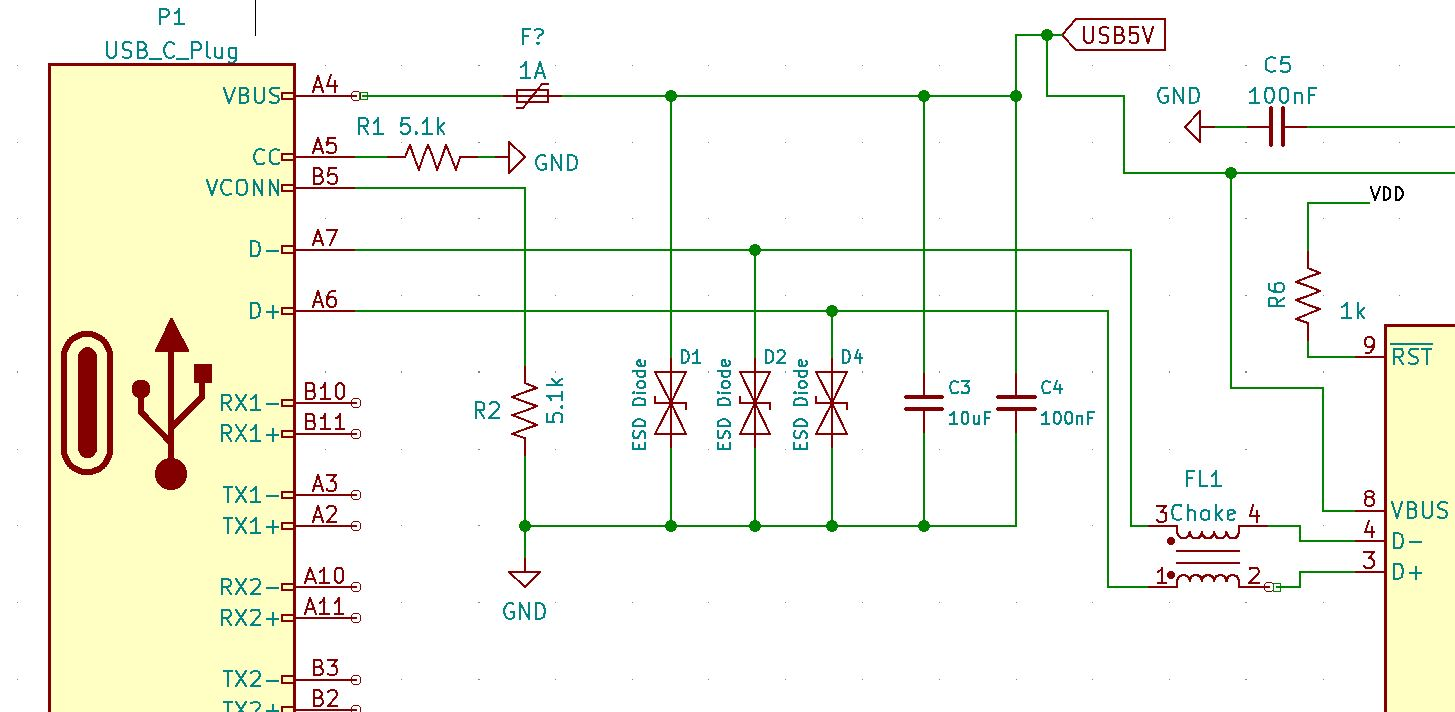
\includegraphics[width=5.5in]{figures/USB-Protection.JPG}
    \caption{USB-C Protection Circuit}
    \label{fig:USB-Protection} 
\end{figure}

\subsubsection{Aether Power Schematic}
\paragraph{Charge Controller} The heart of this power system design is the solar/USB charge controller MCP73871. One of the biggest concerns with designing a solar-powered system is preventing the voltage from collapsing when there is a high current draw from the load. A charger is needed that is capable of monitoring the solar panel voltage and ensuring demand stops when the voltage begins to drop. This will prevent the battery from constantly charging and discharging. The MCP73871 uses a pin called VPCC to achieve this. Depending on the voltage input to this pin, the charger makes sure to draw as much current as it can from the solar panel while adjusting the charge rate to maintain a solar panel voltage above the voltage of VPCC. For this design, a VPCC voltage of 4.5V, just above the Li-Io battery voltage, was used. To do this, a voltage divider was implemented using a 270 \kOhm and 100 \kOhm resistor.

Pins 6, 7, and 8 on the MCP73871 controller are used as system status lines. LEDs along with respective resistors are connected to these pins indicating either a low battery output/charging state, a fully charged state, and a power on state. . In accordance with the data sheet of for the MCP73871, pins 3, 4, 9 and 17 were connected to power. PROG1 or pin 13 on the chip layout, is used to determine charge rate of the controller based on the formula of 1000V divided by the resistor value connected to PROG1. In this design, a 2 \kOhm resistor was used, setting a charge rate of 500 mA. This charge rate can be adjusted depending on the resistor value used. THERM pin 5 on the IC is used for the Li-Io temperature monitoring feature of the system. By connecting a 10 \kOhm NTC thermistor to the charge controller it will be able to detect of the battery temperature is too hot or too cold to safely and effectively charge. The battery is connected to battery pin 14 and 16 on MCP73871.

Lastly, pin 1 is the output pin of the charger where the system load is connected to. Most of the micro-controllers and devices used in the Aether node network ideally operate at 3.3V. Therefore a 3.3V output rail from the charger would be most desirable. However, because the solar panel supply voltage can vary up to 6V in bright daylight conditions, provisions needed to be set so that the micro-controllers did not receive a voltage input above their max rating. This was achieved by using the LP2985-3.3 linear dropout (LDO) regulator. By properly connecting the pins with the appropriate capacitors listed in the data sheet for the LDO,varying output voltages from the MCP73871 could be converted to always output a consistent 3.3V rail. This 3.3V rail will serve as the main power rail in the system. When higher or lower voltages are needed for other system components, the appropriate circuitry will be set in place to achieve the desired voltage. The overall Aether solar/USB charging and power circuit can be seen in Figure \ref{fig:power_schematic}.
\paragraph{USB-UART Bridge}
Another design section of Aether's power system is the IC used to translate USB communication data to UART interface. This is essential because host communication and software implementation will be done through USB input. However, Lora-E5 will only take UART, therefore a conversion IC is needed. This design uses Silicon Lab's USBXpress™ Family CP2102N chip. The Data(D-) and Data(D+) pins on the bridge are connected to the same pins on the USB and are separated by the protection circuit previously discussed. The TX and RX pins are connected to the USB serial RX and TX pins on the micro-controller. LED diodes are set in place to indicate a proper communication link has been established. The features of the CP210N chip eleimantes the need of firmware and driver development and provides a simple and quick method for USB connectivity.
\paragraph{Boost Converter}
A 5V input is needed to properly power Sensirion's Particulate Matter Sensor. The main power line in the circuit is 3.3V since that's what the majority of the chips use. To get a 5V output the LTC3525-5 DC/DC Boost converter was used with the Li-Io battery as the source voltage. The battery was used for Vin instead of the 3.3V power rail because it provides greater efficiency. Perhaps the most crucial feature of this power subsytem is the remote shutdown feature that will be used to turn off the converter, essentially turning off the particulate matter sensor. The SHDN pin is connected with a pull-down resistor to a GPIO pin on the micro controller that will be able to remotely deactivate the sensor when the system wants to enter a low-power operating mode. 

\begin{sidewaysfigure}
    \centering
    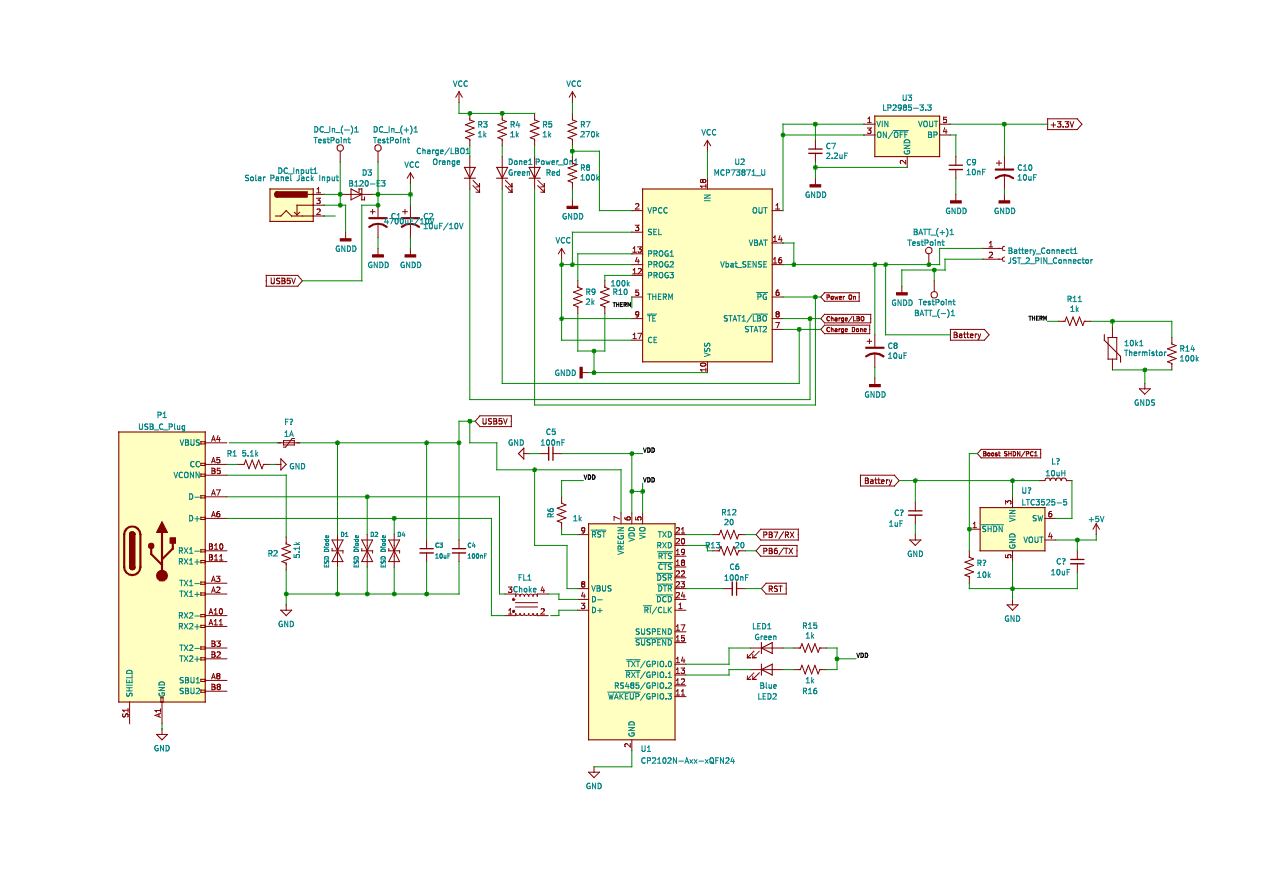
\includegraphics[scale=0.5]{figures/Power_Schematic.jpg}
    \caption{Schematic for Aether node power system}
    \label{fig:power_schematic} 
\end{sidewaysfigure}
